% Created 2022-02-02 Wed 16:11
\documentclass[12pt]{article}
\usepackage[utf8]{inputenc}
\usepackage[T1]{fontenc}
\usepackage{graphicx}
\usepackage{grffile}
\usepackage{longtable}
\usepackage{wrapfig}
\usepackage{rotating}
\usepackage[normalem]{ulem}
\usepackage{amsmath}
\usepackage{textcomp}
\usepackage{amssymb}
\usepackage{capt-of}
\usepackage{hyperref}
\usepackage[usenames,dvipsnames,figures]{xcolor}
\usepackage[autostyle]{csquotes}
\usepackage[final]{pdfpages}
\usepackage{amsfonts, amssymb}            % Math symbols
\usepackage[top=3cm, bottom=3cm, left=3cm, right=3cm]{geometry}
\usepackage{parskip}
\usepackage[natbib=true]{biblatex} \DeclareFieldFormat{apacase}{#1} \addbibresource{~/Documents/Git/msc_thesis/thesis/refs.bib}
\nocite{*}
\hypersetup{colorlinks=false, linkcolor=black, citecolor=black, filecolor=black, urlcolor=black}
\newtheorem{definition}{Definition}[section]
\author{Philip Hartout}
\date{Monday January 24, 2022}
\title{Research notes on metrics for GNNs applied to biological problems}
\hypersetup{
 pdfauthor={Philip Hartout},
 pdftitle={Research notes on metrics for GNNs applied to biological problems},
 pdfkeywords={},
 pdfsubject={},
 pdfcreator={Emacs 27.2 (Org mode 9.4.4)},
 pdflang={English}}
\begin{document}

\maketitle

\section{Graph Neural Networks}
\label{sec:org0a12569}
\subsection{Reviews}
\label{sec:org2845576}
\subsubsection{Graph neural networks:}
\label{sec:org4c781ce}
    A review of methods and applications
Zhou et al mention several GNN approaches in use today
Generative models popular today:
\paragraph{Sequential graph generation process}
\label{sec:org38c0b05}
\begin{itemize}
\item GraphRNN - generates the adjacency matrix of a graph by generating the adjacency vector of each node step by step, with graph outputs with different number of nodes.
\item Li 2018 - also generates nodes and edges sequentially uses the hidden state to decide what to do at the next step
\item GraphAF - also a sequential process, Conducts a validity check of each molecule generated at each step to see if it's valid.
\end{itemize}
\paragraph{Non-sequential graph generation process}
\label{sec:orgf1af366}
\begin{itemize}
\item MolGAN - to generate small molecules. Uses a permutation-invariant to solve the node adjacency matrix at once. Also implements an RL-based optimization toward desired chemical properties
\item Ma et al 2018 - constrained VAE for semantic validity of generated graph
\item GCPN similar to MolGAN, uses RL based methods to ensure validity of domain-specific rules Example work showing EMD kernel:
\item Graph Normalizing Flows
\end{itemize}
This one has a fairly comprehensive website: \url{https://sites.google.com/view/graph-normalizing-flows/}
Full architecture

\begin{figure}[htbp]
\centering
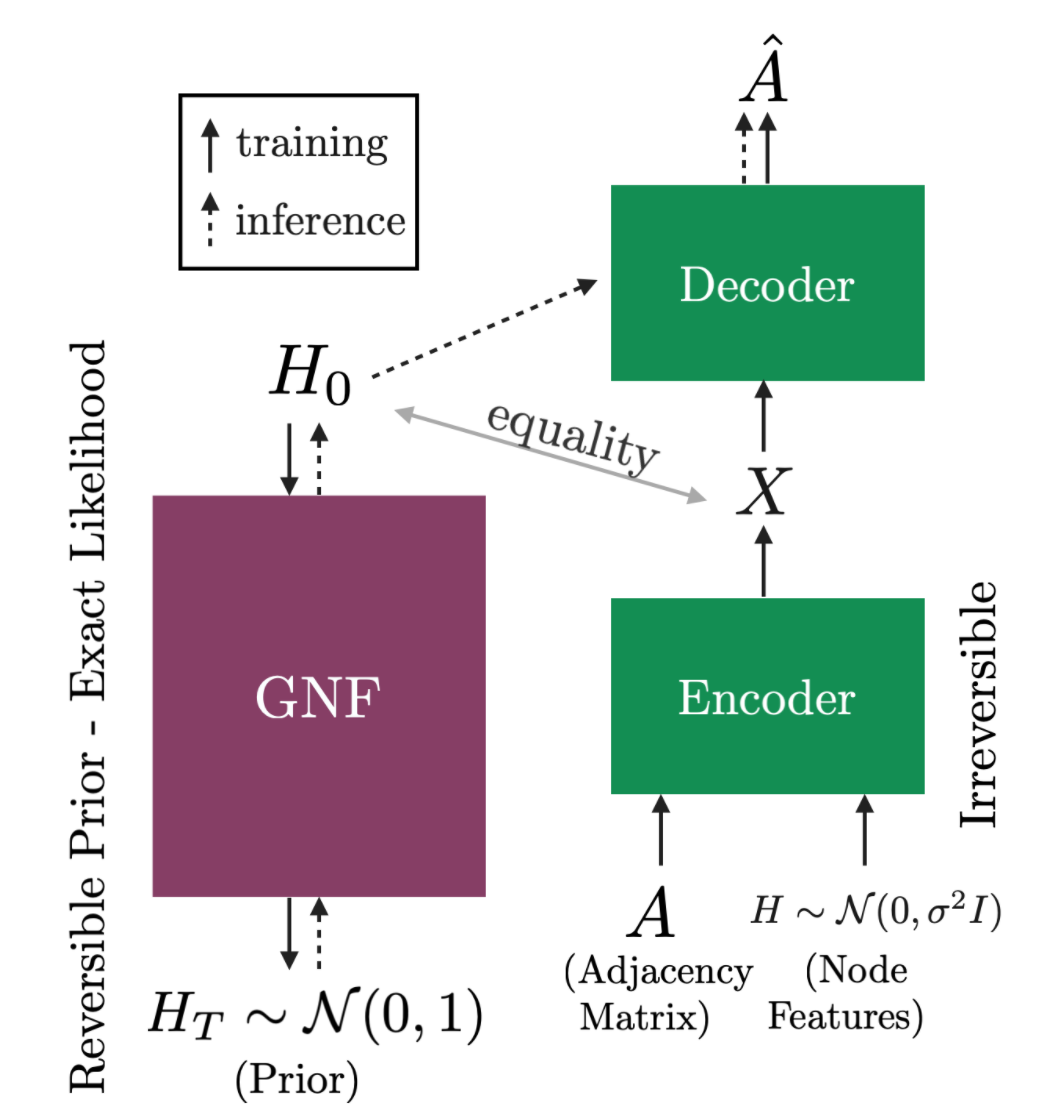
\includegraphics[width=2.0in]{./images/full_arch_gnf.png}
\caption{\label{fig:Full architecture of the graph noramlizing flow DNN}figure name}
\end{figure}
\begin{itemize}
\item Graphite isotropic gaussian for VAE + iterative refinement for decoding
\end{itemize}
\subsection{Three most popular according to O'Bray 2021:}
\label{sec:org34a27ab}
\begin{itemize}
\item GraphRNN, GRAN, Graph Score Matching.

\item Graph Recurrent Attention Networks
\begin{quote}
In previous work, You et al. [37] computed degree distributions, clustering
coefficient distributions, and the number of occurrence of all orbits with 4
nodes, and then used the maximum mean discrepancy (MMD) over these graph
statistics, relying on Gaussian kernels with the first Wasserstein distance,
i.e., earth mover’s distance (EMD), in the MMD.In practice, we found computing
this MMD with the Gaussian EMD kernel to be very slow for moderately large
graphs. Therefore, we use the total variation (TV) distance, which greatly
speeds up the evaluation and is still consistent with EMD. In addition to the
node degree, clustering coefficient and orbit counts (used by [36]), we also
compare the spectra of the graphs by computing the eigenvalues of the
normalized graph Laplacian (quantized to approximate a probability density).
This spectral comparison provides a view of the global graph properties,
whereas the previous metrics focus on local graph statistics.
\end{quote}

\item Graph Score Matching
On MMD, they say the following:
\end{itemize}
\begin{figure}[htbp]
\centering
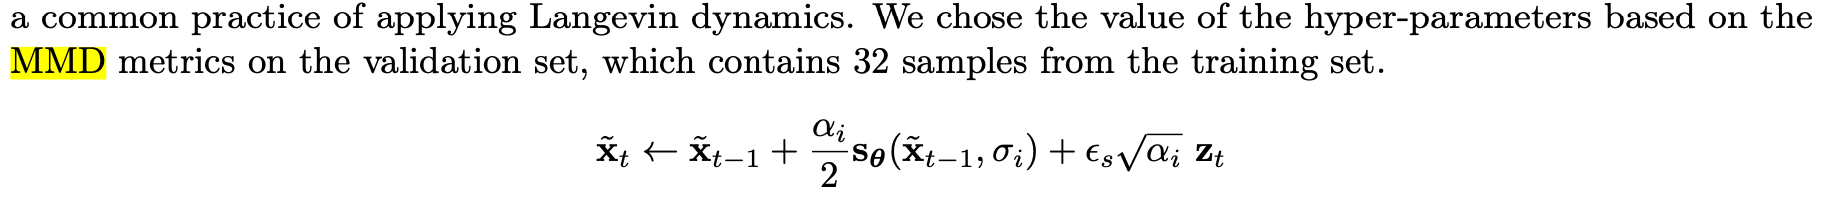
\includegraphics[width=\linewidth]{./images/MMD_settings_graph_score_matching_paper.png}
\caption{\label{fig:MMD settings for evaluation of the graph score matching model}MMD optimization strategy}
\end{figure}

\section{Generative modelling metrics}
\label{sec:org18f08a7}
\subsection{Objective:}
\label{sec:org80c6c46}
\subsubsection{Generative graph dist close to the input graph dist}
\label{sec:orgbcd2db5}
\subsubsection{(pseudo)-metric to assess dissimilarity between G (generated graphs) and G* (input graphs)}
\label{sec:org3c2903f}
\subsection{On images}
\label{sec:org7b32362}
\subsubsection{Frechet Inception Distance}
\label{sec:org1441abc}
The idea here is to use deeper representational layers of an ANN and used the squared Wasserstein metric to compare two multinomial Gaussians.
Introduced 2017
\subsubsection{LPIPS \href{https://richzhang.github.io/PerceptualSimilarity/}{Project page}}
\label{sec:orgef55e67}
Introduced 2017
\subsubsection{Why comparing graphs is hard:}
\label{sec:org4228fdf}
\begin{itemize}
\item Metrics need to deal with spatial invariances such as cycles.
\item Graph edit distance is NP-hard (Zeng 2009) and therefore does not satisfy efficiency criterion.
\item Other publications:
\end{itemize}
\subsection{Desiderata for good metrics:}
\label{sec:org20cc667}
\begin{enumerate}
\item Robust to noise
\item Expressive, if they don't arise from the same dist, then metric should detect this.
\item Computationally efficient.
\end{enumerate}
\section{MMD - current accepted method to evaluate generative GNNs}
\label{sec:org5c236b1}
\begin{itemize}
\item The MMD formula goes as follows:
\end{itemize}
\(\text{MMD}(X, Y) := {1\over n^2} \sum_{i,j=1}^{n}k(x_i, x_j) + {1\over m^2} \sum_{i,j=1}^{n}k(y_i, y_j) - {2\over nm} \sum_{i=1}^{n}\sum_{j=1}^{m}k(y_i, y_j)\)
\begin{itemize}
\item use it for hypothesis/two-sample testing.
\item In practice, we evaluate \(d_{MMD}(\mathcal{G},\mathcal{G*}) :=
  MMD(f(\mathcal{G}),f(\mathcal{G}*))\) for a distribution \(\mathcal{G}\). Given
multiple distributions \(G_1, G_2, \hdots\), the values of \(d_{MMD}\) can be used
to rank models, where smaller values are assumed to indicate a larger
agreement with the original distribution \(\mathcal{G}*\).
\item Commonly used kernels: first Wasserstein distance, total variation distance,
radial basis function.
\item Commonly used descriptor functions: degree distribution histogram, clustering
coefficient, Laplacian spectrum histogram.
\item Recommended kernels: RBF, Laplacian kernel, linear kernel (expressivity \& robustness need to be analyzed)
\end{itemize}
\subsection{Potential pitfalls of descriptors}
\label{sec:orga10a6cd}
\begin{itemize}
\item Degree distributions are ok seemingly
\item Clustering does not distinguish fully connected vs disconnected cliques
\item Spectral methods are not clearly expressive. Does not seem to be for certain classes of graphs.
\item Parameters and descriptors are set a priori in the best case
\item Model performance is highly dependent on parameters and descriptor functions.
\end{itemize}
\section{Research objectives}
\label{sec:orge4418bb}
There are multiple objectives here:
\begin{enumerate}
\item Find optimal kernel/hyperparameter combination based on controlled experiments on a given dataset to evaluate a good MMD configuration.
\begin{itemize}
\item For this we will need \url{https://www.alphafold.ebi.ac.uk/download}, because it's clean. Also filter single chain proteins to extract graphs in the first place.
\item This can be built as a first step to get the pipeline going.
\end{itemize}

\item Show which parameters influence evaluation and how?
\begin{itemize}
\item Conduct perturbation experiments on graphs
\end{itemize}

\item Find novel domain-agnostic evaluation \& domain-specific evaluation metrics
\begin{enumerate}
\item Domain-agnostic evaluation measures
\begin{itemize}
\item Correlation with graph-edit distance
\item Correlation with perturbation
\item Topology/persistence based approaches could be useful for modelling features like binding pockets, etc?
\end{itemize}

\item Domain-specific evaluation measures
\begin{itemize}
\item Alignment
\item Energy?
\end{itemize}
\end{enumerate}
\end{enumerate}
\subsection{From Tim: gather literature sources. Intro structure}
\label{sec:org3d7a487}
\subsubsection{Evaluation of generative models (different domains)}
\label{sec:org7833772}
\subsubsection{Evaluation of generative models for graphs}
\label{sec:orgd96e491}
\paragraph{Check how it was done before, why combo of parameters/kernels were used.}
\label{sec:org45ebe8c}
\subsubsection{Evaluation of proteins (…/molecules/drugs) (What makes a valid protein?)}
\label{sec:org0a7ea03}
\subsubsection{Evaluation of generative models for proteins}
\label{sec:org9934110}
\section{Module-wise breakdown of the plan}
\label{sec:org2a8afbe}
\begin{itemize}
\item Graph extraction
\item Descriptor functions
\item kernels, MMD
\item Domain agnostic
\item Domain specific
\item Other metrics
\item TDA descriptors
\item Labeled edge graph
\item NSPDK
\item Other metrics
\item Extract graph from real datasets
\end{itemize}
\section{Annotations}
\label{sec:org0a5e2f1}
Online approach to k-NN graph construction
epsilon nearest neighbor graphs dissertation with history and construction methods.
Giotto-TDA library
Heat kernel on persistence diagrams
original mmd papers
Specific MMD for biological data:
Introduction several metrics based on the features extracted by an untrained random GNN, showing more expressive metrics of GNN performance
Neighborhood Subgraph Pairwise Distance graph kernel (NSPDK)
Examples using the Neighborhood Subgraph Pairwise Distance graph kernel (NSPDK)
Inverse protein folding problem, maybe good to look at to see what makes a good protein.
Papers discussing Delaunay graphs (dual graph of Voronoi diagram), obtained through Delaunay triangulation. Useful for extracting hierarchical structures. Graph edges can also be added on the basis of the Delaunay triangulation. Delaunay triangles correspond to joining points that share a face in the 3D Voronoi diagram of the protein structures. For distance-based edges, a Long Interaction Network (LIN) parameter controls the minimum required separation in the amino acid sequence for edge creation. This can be useful in reducing the number of noisy edges under distance-based edge creation schemes. Edge featurisation for atom-level graphs is provided by annotations of bond type and ring status.
Not a great review, but still useful source of references and gives overview of the field.
\section*{References}
\label{sec:org8fed4c4}
\printbibliography
\end{document}
